\documentclass[../../main.tex]{subfiles}
\begin{document}

\begin{problem}
\textbf{最大间隙问题}

给定 $n$ 个实数$x_1, x_2, \cdots, x_n$,求这$n$个实数在数轴上相邻2个数之间的最大差值。
直观解法:将$ n $个数排序后计算间距,再找最大值。
假设对任何实数的下取整函数耗时$O(1)$,设计解最大间隙问题的线性时间算法。

算法输入:输入数据由文件名 \verb|input.txt| 的文本提供。
文件的第一行有一个正整数 n ,接下来有 n 个实数。

算法输出:将找到的最大间隙输出到文件 \verb|output.txt| 中。
\end{problem}

\begin{solution}
算法的主要思路为:
\begin{itemize}
    \item 检查数组大小:如果数组的大小小于2,直接返回0,因为没有间隔可言。
    \item 找到数组中的最大值和最小值:使用 \verb|Find_Max_Min| 方法找到数组中的最大值和最小值。
    \item 计算每个桶的间隔:计算每个桶的间隔 \verb|interval|,公式为$(\text{最大值} - \text{最小值}) / (\text{数组大小}-1)$,
    从而保证桶间的间距一定大于桶内的间距。
    \item 初始化桶:创建一个桶的向量,每个桶是一个三元组,包含最小值、最大值和一个布尔值（表示桶是否被使用）。
    \item 将每个元素分配到桶中:遍历数组中的每个元素,计算其对应的桶索引,并更新桶的最小值和最大值。
\end{itemize}
最后就可以遍历桶,计算相邻桶之间的最大间隔从而得出结果。

该算法完整代码如下:    
\inputminted[
    frame=lines,
    framesep=2mm,
    baselinestretch=1.2,
    fontsize=\footnotesize
]{cpp}{project/project_1/src/main.cpp}

运行代码前,需要将输入数据写入 \verb|input.txt| 文件中,如下图所示:
\begin{figure}[htb]
    \centering
    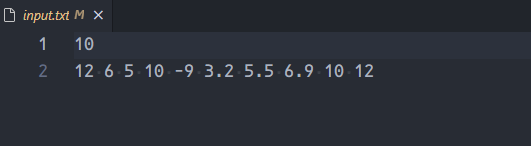
\includegraphics[width=450pt]{figure/Figure_1_1.png}
    \caption{input.txt 文件}
\end{figure}
\newpage
运行后,得到的 \verb|output.txt| 文件如下:
\begin{figure}[htb]
    \centering
    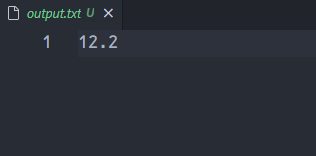
\includegraphics[width=450pt]{figure/Figure_1_2.png}
    \caption{output.txt 文件}
\end{figure}
\end{solution}

\end{document}